\section{Blockchain Objects}\label{sec:impl-objects}

In \iblock{}, the two main data structures representing the Bitcoin network
state are the blockchain and the mempool. These are composed of two core object
types: \code{Block} and \code{Transaction} objects.

These objects, along with their composite elements, are defined using
\omnetpp{}'s \emph{message definition} language. This setup allows to
incorporate these objects directly into messages and NED files, enabling them
to be analyzed and modified within the \omnetpp{} QT environment.

Objects in \iblock{} inherit from base classes that include essential
attributes, such as the object hash and size. \figref{fig:objects-uml} presents
the UML diagram of the objects in \iblock{}, with a focus on their base
classes.

\begin{figure}[tbhp]
	\centering
	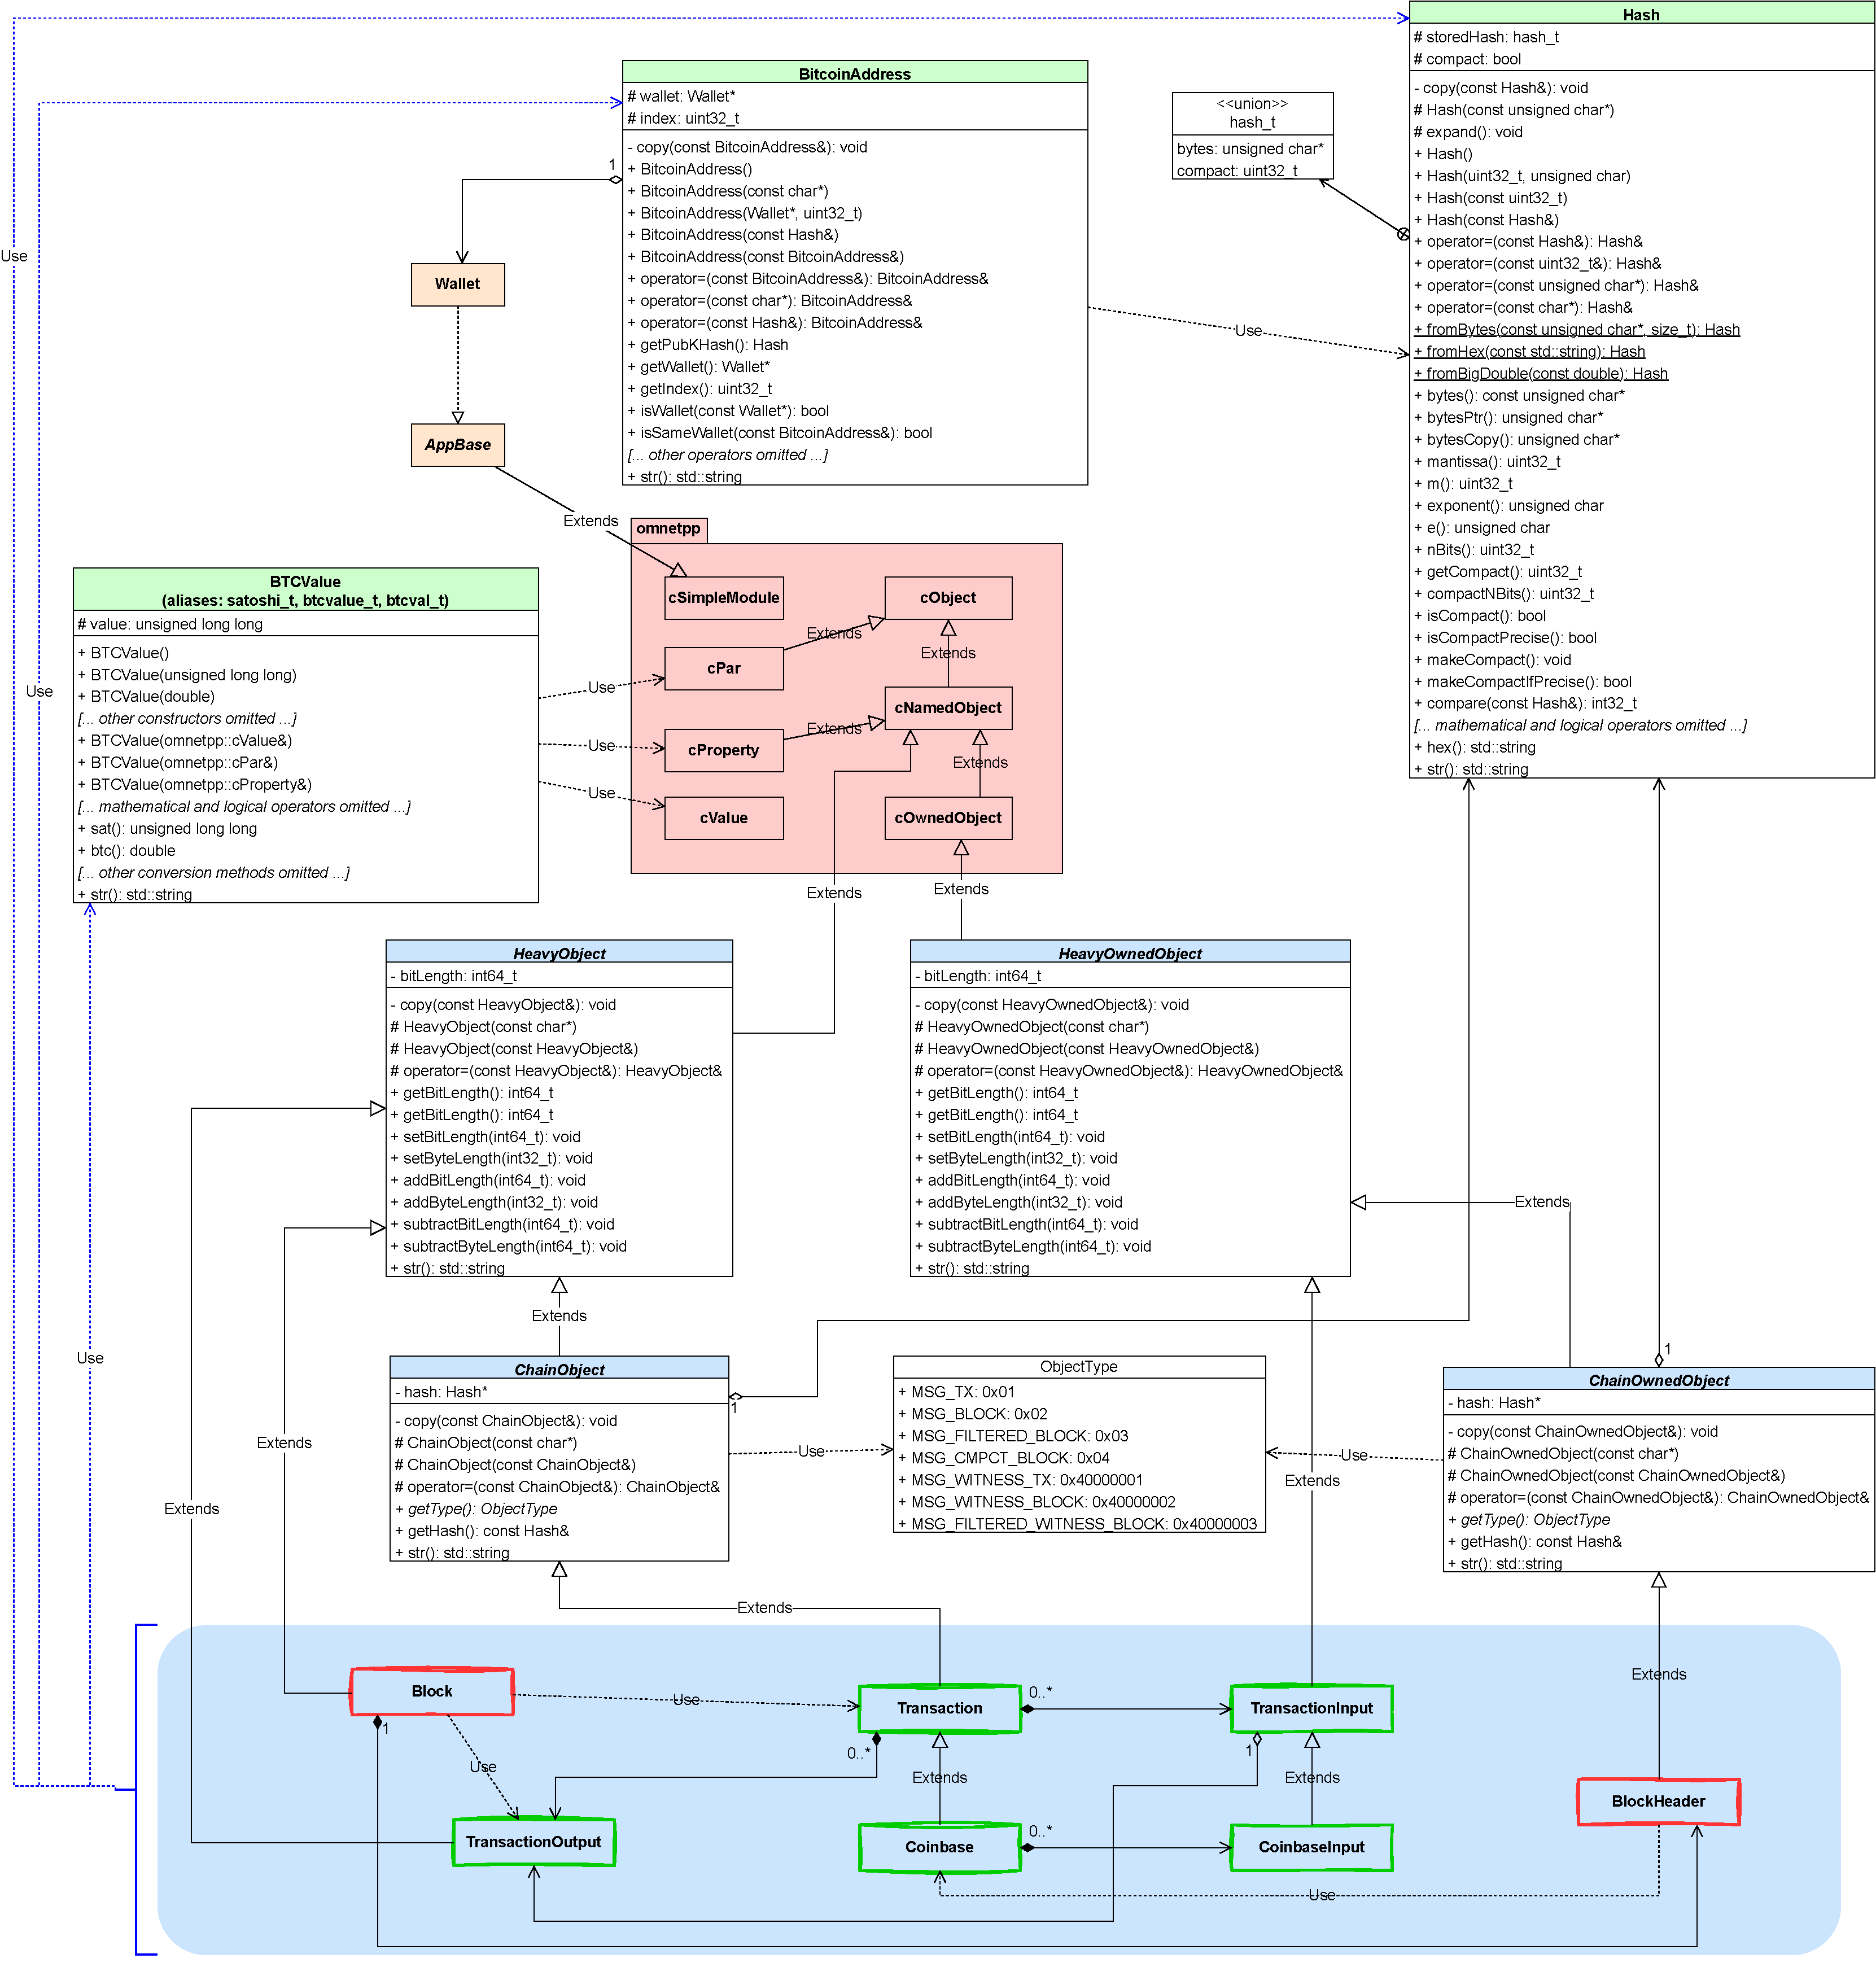
\includegraphics[width=\textwidth]{img/objects-uml}
	\caption{UML diagram of the objects in \iblock{}, highlighting base and
	utility classes. Classes within the blue area represent the core
	objects utilized by the simulation model.}\label{fig:objects-uml}
\end{figure}

\subsection{HeavyObject}\label{subsec:impl-heavyobject}

The \code{HeavyObject} class represents objects with a defined size in bits.
This class inherits from \omnetpp{}'s \code{cNamedObject} class, classifying it
as a \emph{non-owned} object --- meaning no other entity claims ownership of
it. By contrast, the \code{HeavyOwnedObject} class, derived from
\code{cOwnedObject}, is intended for objects with a designated owner.

Ownership in \omnetpp{} supports memory management and sanity checks. When an
object is owned by another, the owner assumes responsibility for its deletion.
Additionally, certain actions, such as sending the object within a message, are
restricted to the owner.

In this structure, the \code{Block} and \code{TransactionOutput} classes extend
\code{HeavyObject}, while the \code{TransactionInput} class derives from
\code{HeavyOwnedObject}. Transaction inputs are always owned by the
\code{Transaction} object they belong to.

\subsection{ChainObject}\label{subsec:impl-chainobject}

The \code{ChainObject} class, derived from \code{HeavyObject}, represents
essential blockchain objects like block headers and transactions. Its
counterpart, \code{ChainOwnedObject}, is derived from \code{HeavyOwnedObject}.

Each \code{ChainObject} has a unique identifier represented by its hash. While
the hash is not actively used in simulation operations, it can be helpful for
debugging and visual inspection within the \omnetpp{}'s QT environment.

Within the class hierarchy, \code{Transaction} is derived from
\code{ChainObject}, while \code{BlockHeader} is derived from
\code{ChainOwnedObject}. Unlike these, the \code{Block} class is based directly
on \code{HeavyObject} rather than \code{ChainObject} --- this is to support
\emph{inventory} messages, which, in the Bitcoin protocol, announce new blocks
using the block header hash rather than the complete block hash. The specific
type of each chain object is defined through the \code{ObjectType} enumeration.

\subsection{Utility Classes}\label{subsec:impl-utility}

There are three utility classes used to support core blockchain functionality
in \iblock{}: \code{Hash}, \code{BitcoinAddress}, and \code{BTCValue}.

\subsubsection{Hash}\label{subsubsec:impl-hash}

The \code{Hash} class enables hash representation, supporting both extended
format (32 bytes) and \emph{compact} format (4 bytes). It is also used to
represent the \emph{target NBits}, the threshold value that a block's hash must
meet to satisfy Proof-of-Work validation.

In Bitcoin and \iblock{}, compact hash format condenses a 256-bit hash into 4
bytes, with the three least significant bytes representing the \emph{mantissa}
and the most significant byte representing the \emph{exponent}. The conversion
from compact to full hash format is shown in \eqref{eq:compact2hash}, where
\(M\) is the mantissa, and \(E\) is the exponent.

\begin{equation}\label{eq:compact2hash}
	H = M \times 256^{(E - 3)}
\end{equation}

Bitcoin treats the mantissa as a signed integer, and \iblock{} adheres to this
convention as well \cite{bitcoin-dev}. If the mantissa is negative, the compact
representation can be adjusted by dividing the mantissa by 256 and increasing
the exponent by one, which yields an equivalent value with a different
encoding. The \code{Hash} class performs this adjustment automatically.

\subsubsection{BitcoinAddress}\label{subsubsec:impl-bitcoinaddress}

In \iblock{}, Bitcoin addresses are represented by a pointer to the owning
\code{Wallet} module and an integer index, allowing each \code{Wallet} to hold
multiple addresses. The \code{BitcoinAddress} class also provides methods to
retrieve a hash that uniquely represents the address.

\subsubsection{BTCValue}\label{subsubsec:impl-btcvalue}

The \code{BTCValue} class enables configuration and NED files to represent
Bitcoin amounts in various units, such as BTC (Bitcoins), mBTC
(milli-bitcoins), and satoshis (\(10^{-8}\) BTC). Internally, values are stored
in satoshis, Bitcoin's smallest unit. The class includes multiple \emph{getter}
methods for retrieving amounts in different units.

This class also facilitates extraction of values from NED parameters and
properties by directly assigning the parameter or property to a \code{BTCValue}
object. Additionally, it supports a wide range of mathematical and logical
operations.

\subsection{Modeling Transactions}\label{subsec:impl-transactions}

In \iblock{}, transactions are represented by the \code{Transaction} class. The
structure and composition of this class are illustrated in
\figref{fig:transaction-uml}.

\begin{figure}[tbhp]
	\centering
	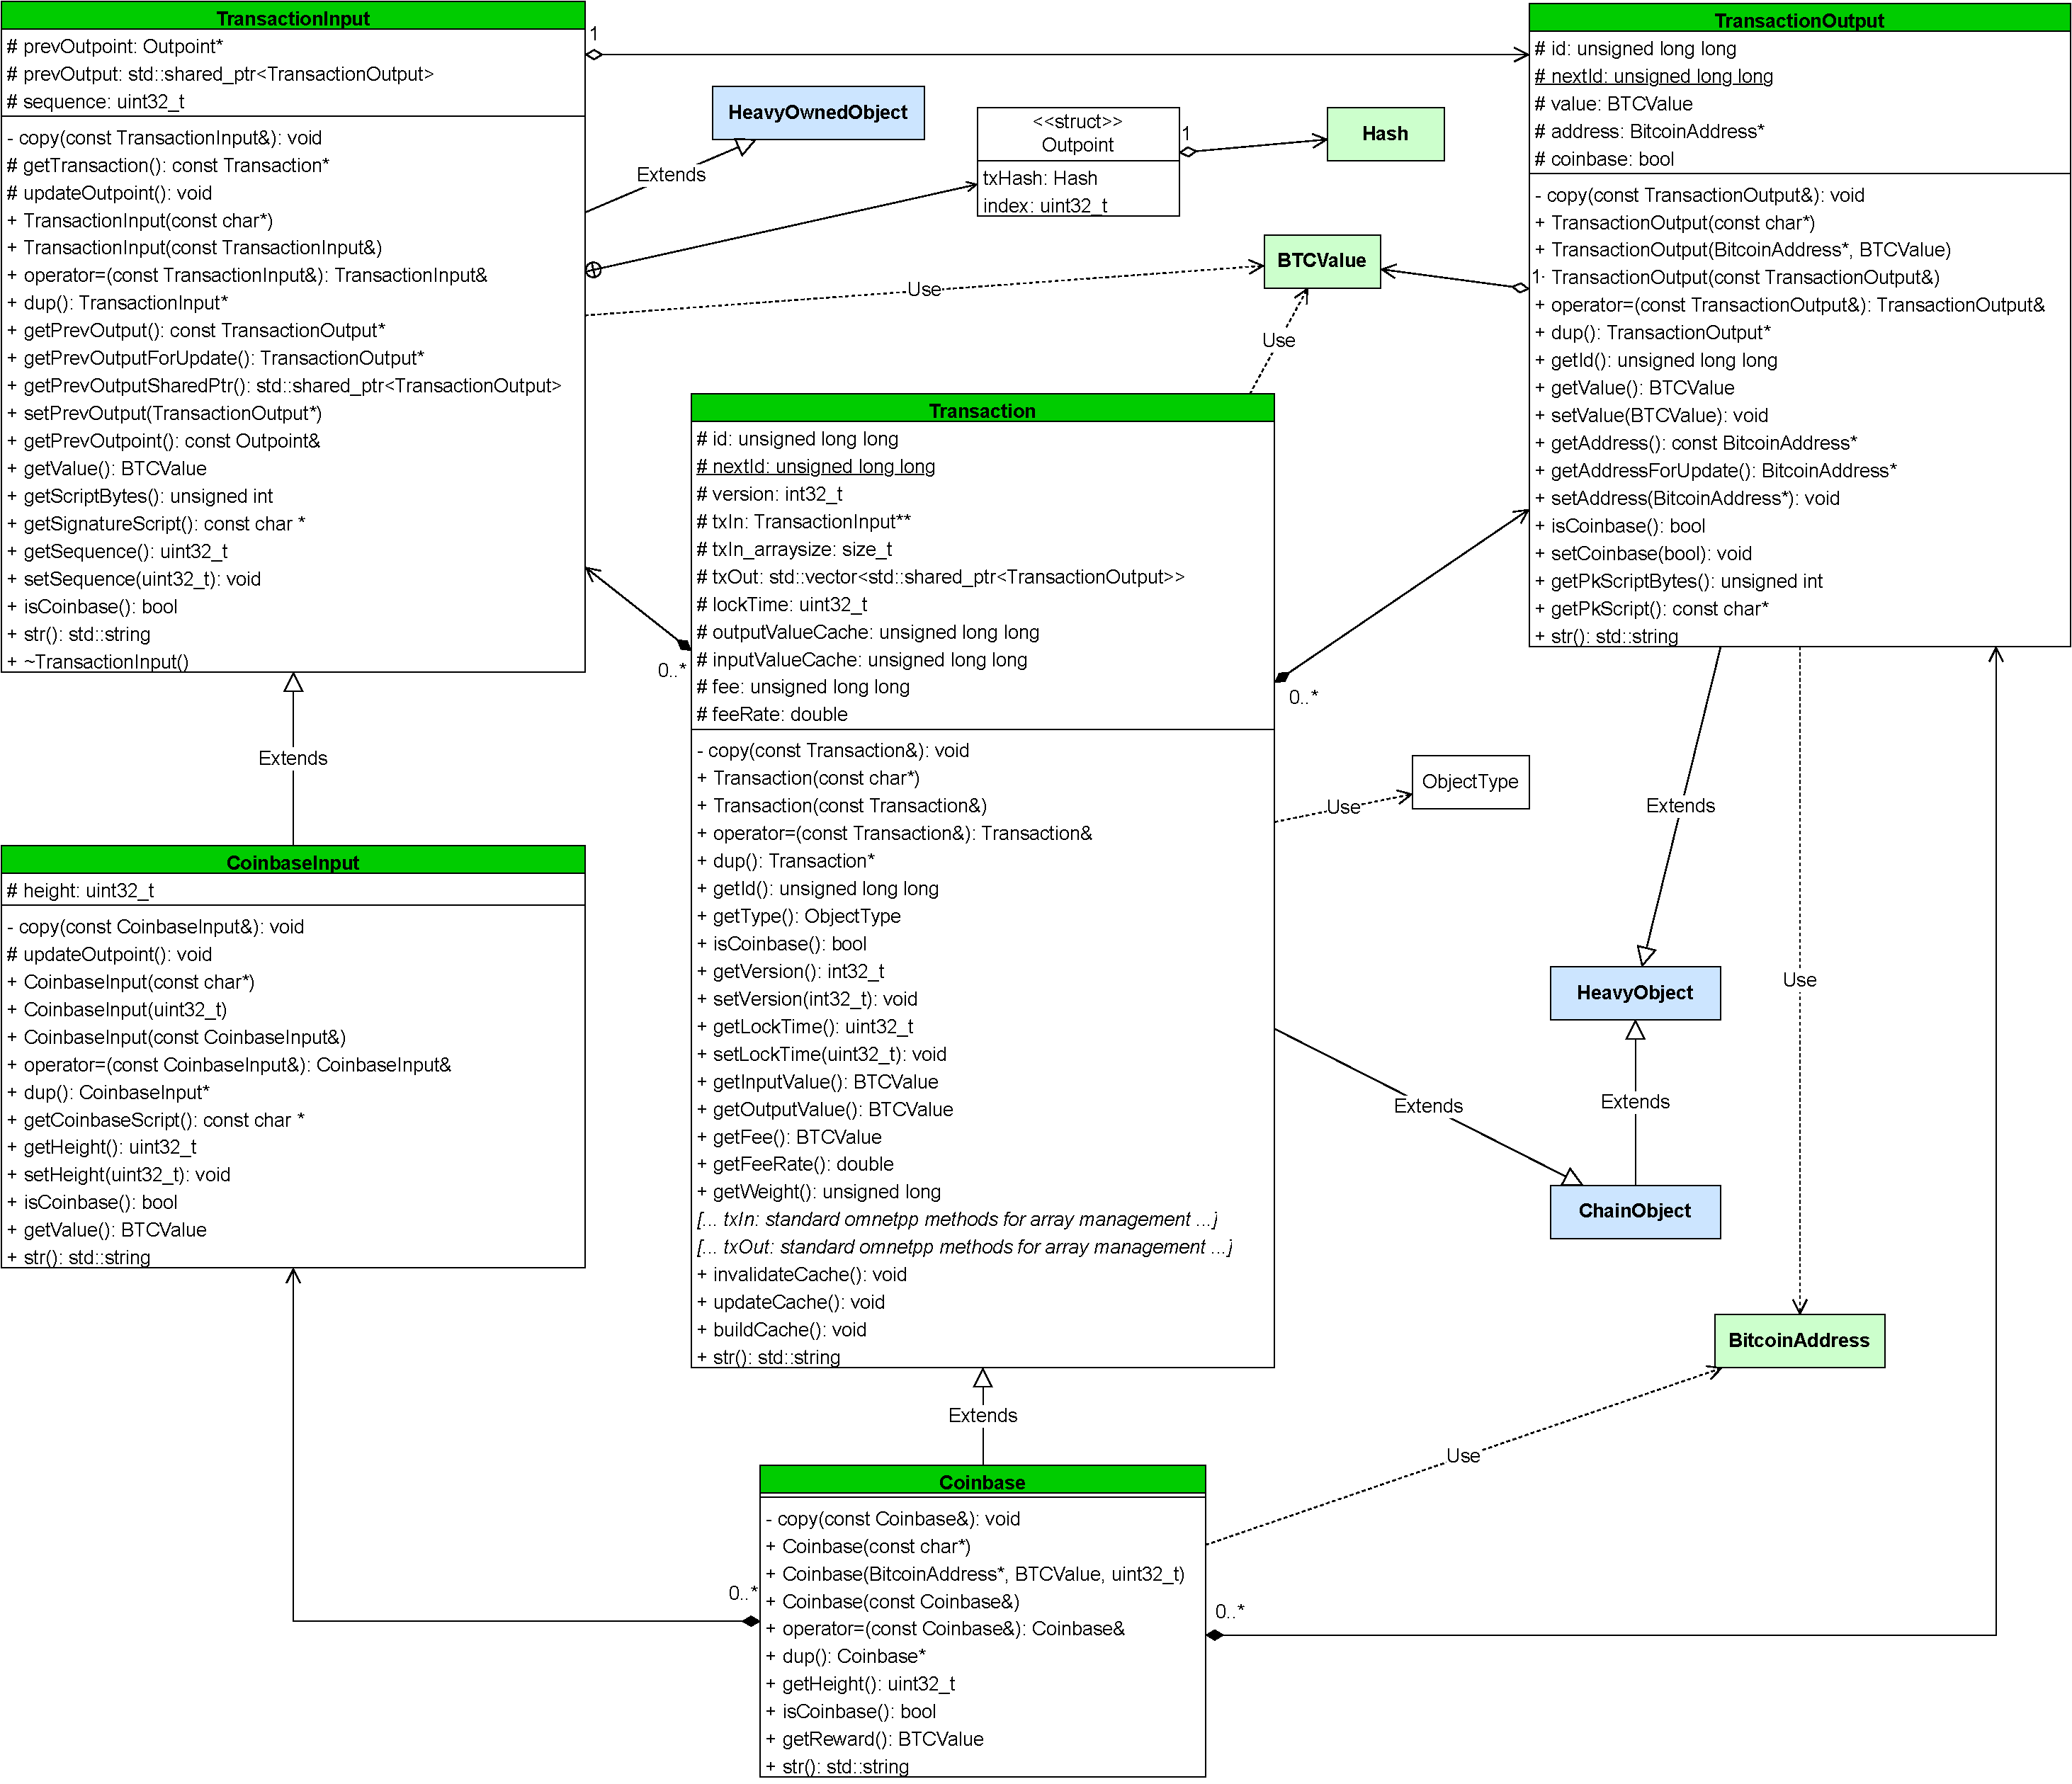
\includegraphics[width=\textwidth]{img/transaction-uml}
	\caption{UML diagram of the \code{Transaction} class and its component
	classes.}\label{fig:transaction-uml}
\end{figure}

Following the Bitcoin protocol, each \code{Transaction} consists of multiple
inputs (\code{TransactionInput}) and outputs (\code{TransactionOutput}). Each
\code{TransactionInput} refers to a specific \code{TransactionOutput} from a
prior transaction.

The \code{Coinbase} class extends \code{Transaction} to represent a coinbase
transaction, which is used to reward miners. This transaction includes a single
special input, \code{CoinbaseInput}, which does not reference any previous
output.

\iblock{} transactions incorporate all fields supported by the Bitcoin
protocol. Additionally, certain fields in the \code{Transaction} class act as a
\emph{cache}, storing values computed from other fields. These optimizations
are covered in \secref{sec:optimizations}.

Memory management is handled with \emph{smart pointers} to maintain efficient
references. For instance, references to transaction outputs are stored as smart
pointers, as they are shared across different components: each \code{Wallet}
maintains a list of unspent transaction outputs (instances of
\code{TransactionOutput}), each transaction input references a prior output,
and UTXO lists are also stored within the \code{Block} object for performance
reasons.

\subsection{Modeling Blocks and the Blockchain}\label{subsec:impl-blocks}

\figref{fig:block-uml} presents the UML diagram of the \code{Block} and
\code{BlockHeader} classes. Each \code{Block} contains a \code{BlockHeader} and
a list of transactions. The fields in \code{BlockHeader} mirror those in an
actual Bitcoin block header.

\begin{figure}[tbhp]
	\centering
	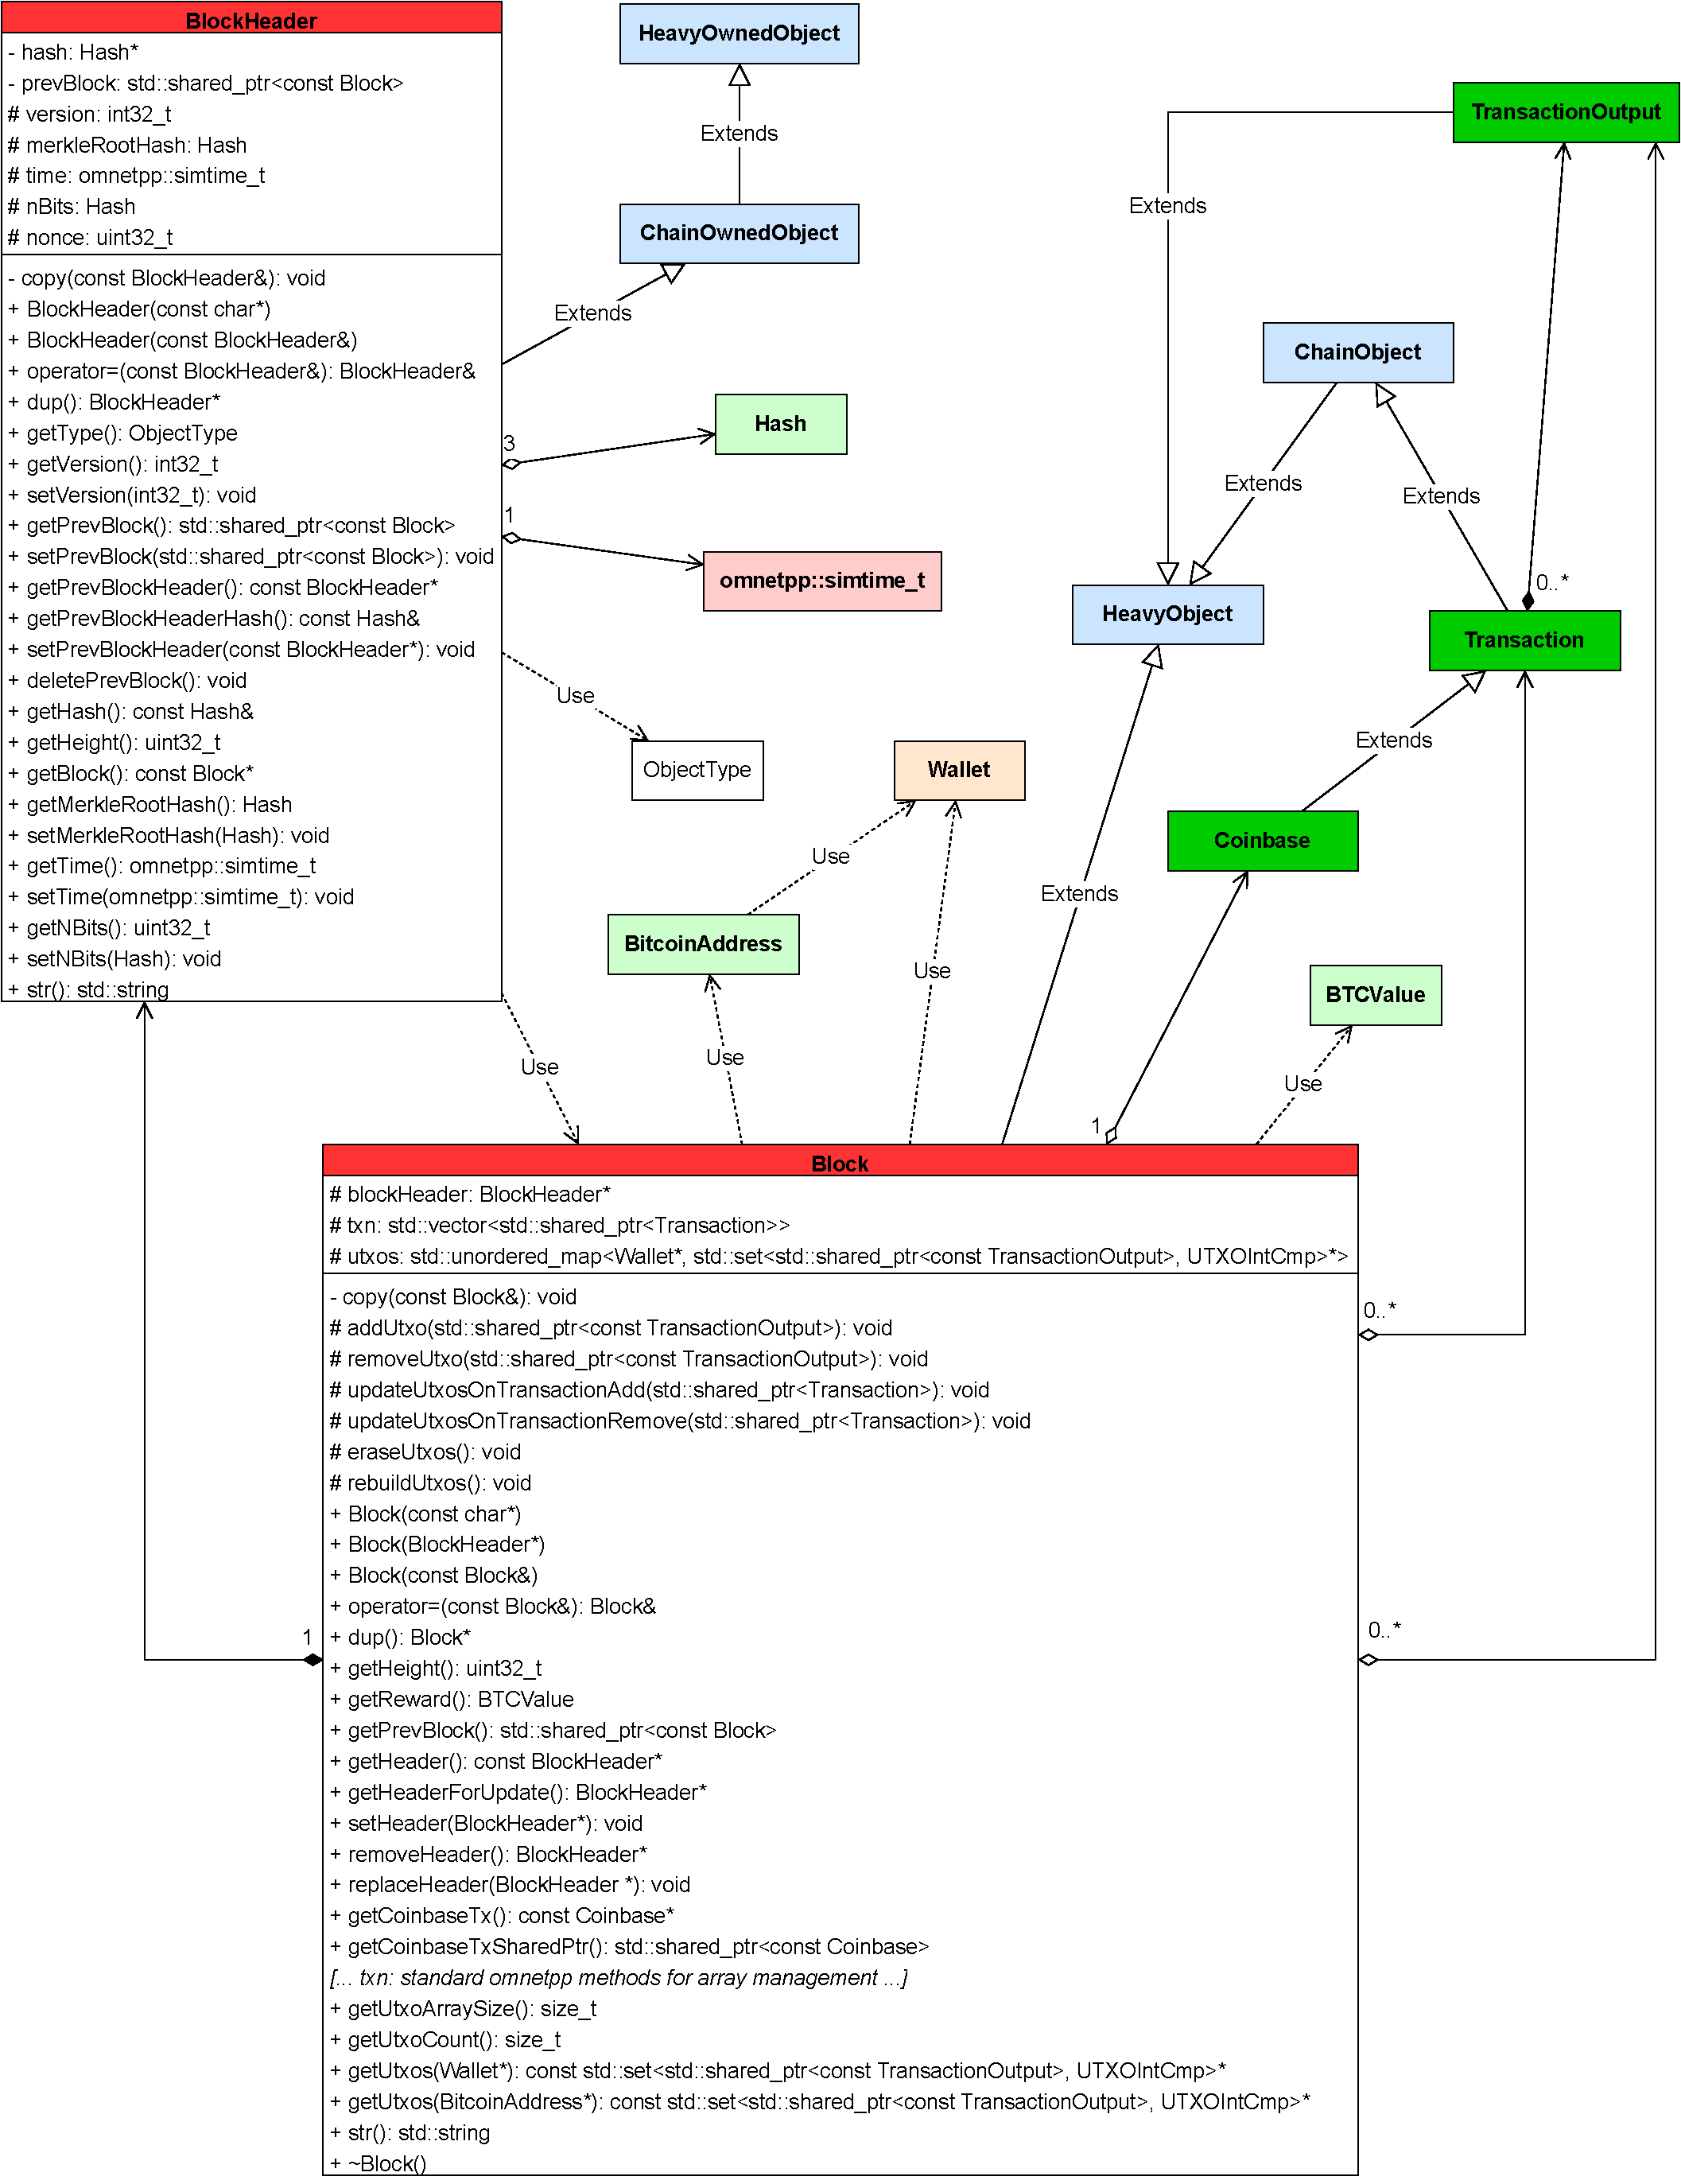
\includegraphics[width=\textwidth]{img/block-uml}
	\caption{UML diagram of the \code{Block} and \code{BlockHeader}
	classes.}\label{fig:block-uml}
\end{figure}

The \code{Block} class maintains an updated list of UTXOs (Unspent Transaction
Outputs), which is built as transactions are added to the block. This process
takes UTXOs from the previous block, removes spent outputs, and adds new ones
from current transactions. Nodes rely on this list to retrieve UTXOs for their
wallets, combining them with UTXOs from the mempool.

Blocks are linked through smart pointers held in their headers, which enables
the \code{GBM} (Global Blockchain Manager) to remove obsolete blocks from
memory efficiently. Transactions are also referenced by smart pointers,
ensuring that if a block is deleted, its transactions are also removed ---
unless referenced elsewhere, such as by other blocks or a node's mempool.
